\documentclass[../template]{subfiles}

\begin{document}
\section{Matching}
\subsection{Definizione di Matching}
Dato un grafo non orientato $G = (v, A)$, un matching è un sottoinsieme $M \subseteq A$ dell'insieme di archi $A$ tale che
in $M$ non ci siano coppie di archi adiacenti\footnote{Con un nodo in comune}.
\subsection{Matching a peso massimo}
Di tutti i matching possibili, vogliamo trovare quello il cui peso $w(M) = \sum_{e \in M} w_e$ sia massimo.

\begin{figure}[h]
    \centering
    \begin{tikzpicture}[rotate=90]
        \SetGraphUnit{2}
        \Vertices{circle}{6, 3, 4, 5, 1}
        \WE(6){2}
        \Edge[label=$2$](2)(4)
        \Edge[label=$3$](2)(5)

        \tikzset{EdgeStyle/.style={color=green}}
        \Edge[label=$1$](2)(3)
        \Edge[label=$5$](4)(5)
        \Edge[label=$6$](1)(6)

        \tikzset{EdgeStyle/.style={color=red}}
        \Edge[label=$4$](3)(6)
        \Edge[label=$5$](1)(2)
        ;
    \end{tikzpicture}
\end{figure}

\noindent L'insieme di archi $M_1 = \{ (1, 2) \, (3, 6)\}$ forma un matching di peso $9$, mentre $M_2 = \{(2, 3)\,(4, 5)\,(1, 6)\}$ ha un peso
di $12$.
Algoritmi di matching sono utilizzati per determinare accoppiamenti ottimali tra i nodi.
\\[10pt]
Viene detto matching di \textbf{cardinalità massima}, l'insieme di problemi dove il peso di ogni arco è unitario.
In caso di grafi bipartiti, si cerca una soluzione che colleghi i due set di nodi.
\lstinputlisting[firstline=42, lastline=84]{algorithms/matching.py}

%\subsubsection{Matching iniziale}
%\lstinputlisting{algorithms/initial_match.py}
\subsubsection{Complessità}
$O(\min(|V_1|, |V_2|) |A|)$, quindi polinomiale. Ad ogni iterazione la cardinalità del matching incrementa di 1 unità, appena raggiunta la cardinalità
di $V_1$ e $V_2$ termina. Esiste un algoritmo più efficiente di complessità $O(|V|½|A|)$ ma non è trattato nel corso.

\subsubsection{Note}
Collegando un nodo sorgente alla prima classe di partizione, ed un nodo destinazione alla seconda classe, il problema è riconducibile ad un
problema di matching di cardinalità massima.

\subsection{Assegnamento}
Dato un grafo bipartito completo $G = (V_1 \cup V_2, E)$ con $V_1 = \{a_1 \dots a_n\}$ e $V_2 = \{b_1 \dots b_n\}$ ($|V_1| = |V_2|$),
e $\forall (i, j) \in E \quad d_{ij} \ge 0$ ed interi,
il problema d'assegnamento è trovare il matching $M$ di cardinalità $n$ tale per cui
$\sum_{(i, j) \in M} d_{ij}$ è minimo.
\\[10pt]
Il numero di soluzioni ammissibili è ovviamente $n!$, siccome ad ogni nodo nella prima
partizione deve corrispondere un nodo nella seconda.
\\
Nei casi in cui $|V_1| \neq |V_2|$ vengono aggiunti elementi fittizi con collegamenti di costo 0 nell'insieme con meno elementi.

\subsection{Algoritmo Ungherese}
% TODO: Descrizione algoritmo

Presa in ingresso una tabella dei costi $T_0 = d_{ij}$ di ordine $n$ come nel caso in esempio
\ref{tab:hungarian_example}, dove ad ogni lavoratore $a_1 \dots a_n$ è associato costo per lavoro $b_1 \dots b_n$, il
procedimento dell'algoritmo è il seguente:

\begin{table}[h]
    \centering
    \begin{tabular}{|c|cccc|}
        \hline
    & $b_1$ & $b_2$ & $b_3$ & $b_4$\\
    \hline
        $a_1$ & 2 & 3 & 4 & 5\\
        $a_2$ & 6 & 2 & 2 & 2\\
        $a_3$ & 7 & 2 & 3 & 3\\
        $a_4$ & 2 & 3 & 4 & 5\\
        \hline
    \end{tabular}
    \caption{Tabella dei costi d'esempio}
    \label{tab:hungarian_example}
\end{table}

\begin{itemize}
    \item Si calcola il minimo valore presente in ogni colonna: $d^0_j = \min_i d_{ij}$
    \item Per ogni colonna $j$, sottrarre ad ogni suo elemento il valore $d^0_j$ rispettivo
    \item Ripetere la stessa operazione per le righe della matrice, sottraendo il valore $d^1_i = \min_j d_{ij}$ ad ogni
        elemento della riga
\end{itemize}
Seguendo il caso di esempio si ottiene una nuova tabella $T_1$:

\begin{table}[h]
    \centering
    \begin{tabular}{|c|cccc|}
        \hline
    & $b_1$ & $b_2$ & $b_3$ & $b_4$\\
    \hline
        $a_1$ & 0 & 1 & 2 & 3\\
        $a_2$ & 4 & 0 & 0 & 0\\
        $a_3$ & 5 & 0 & 1 & 1\\
        $a_4$ & 0 & 1 & 2 & 3\\
        \hline
    \end{tabular}
    \caption{Tabella $T_1$ dei costi d'esempio}
    \label{tab:hungarian_example_t1}
\end{table}


È importante notare che tutti gli elementi della tabella $T_1 = d_{ij}^2$ dopo queste due operazioni sono strettamente positivi.

Definita la matrice $x_{ij} = 1$ se $(i, j)$ è un assegnamento, 0 altrimenti; la richiesta di assegnamento di uno ed un
solo lavoro per lavoratore è descritta da:
\[
    \sum_{j \in V_2} x_{ij} = 1 \quad \forall i \in V_1 \qquad
    \bigwedge\qquad
    \sum_{i \in V_1} x_{ij} = 1 \quad \forall j \in V_1
\]
Utilizzando queste osservazioni, è possibile ricavare la seguente relazione:
\[
    \sum^n_{i = 1} \sum^n_{j=1} d_{ij} x_{ij} =
    \sum^n_{i=1}\sum^n_{j=1} d_{ij}^2 x_{ij} + \sum_{j=1}^n d_j^0 \sum_{i=1}^n x_{ij}+ \sum^n_{i=1} d_i^1\sum^n_{j=1} x_{ij} =
    \sum^n_{i=1}\sum^n_{j=1} d_{ij}^2 x_{ij} + D_0 + D_1
\]
Dato che la quantità $d_{ij}^2 > 0$ e $x_{ij} > 0$ per ogni coppia $(i, j)$ si ha che:
\[
    \sum^n_{i=1}\sum^n_{j=1} d_{ij} x_{ij}  \ge D_0 + D_1
\]
Nel caso in cui esista una soluzione di peso pari a $D_0$ e $D_1$ essa sarà ottima.
Il problema diventa quindi determinare un sottoinsieme $\Delta$ di cardinalità massima degli 0 nella matrice $T_2$, tale
che presi due elementi qualsiasi, essi siano indipendenti \footnote{appartengano a righe e colonne diverse}.

Se il problema ammette soluzione $\Delta$ tale che $|\Delta| = n$, allora a tale è un assegnamento.
Consideriamo la matrice $x_{ij} = 1$ se $(i, j) \in \Delta$, nel caso in cui $\Delta$ non sia un assegnamento
\[
    \exists j : \sum_{i=1}^n x_{ij} \neq 1
\]
Nel caso in cui $\sum^n_{i=1} x_{ij} = 0$, nessun elemento di $\Delta$ è presente nella colonna $j$, quindi dato che
$|\Delta| = n$ dovranno esserci $n$ elementi nelle rimanenti $n-1$ colonne. Per il principio della piccionaia almeno una
colonna contiene due elementi. Quindi segue l'assurdo dato che gli elementi in $\Delta$ devono essere indipendenti,
quindi devono appartenere a colonne diverse.

Nel caso in cui $\sum^n_{i=1} x_{ij} \ge 2$, in tal caso nella stessa colonna $j$ ci sono 2 o più elementi di $\Delta$
segue l'assurdo identico al caso precedente.
\subsubsection{Calcolo dell'assegnamento $\Delta$}
Dato un grafo $G = (A,B;E)$, con $a_1\dots a_n \in A$ e $b_1 \dots b_n \in B$; tra il vertice $a_i$ ed il vertice $b_j$
si traccia un arco se e solo se $d_{ij}^2 = 0$.

Cercare il massimo insieme di 0 indipendenti equivale a risolvere il problema di matching di massima cardinalità.

Nel nostro caso di esempio quindi otterremo la soluzione
\[
    \Delta = \big\{(a_1, b_1) (a_2, b_3) (a_3, b_2)\big\}
\]
tale per cui $|\Delta| = 4$ quindi $|\Delta| < n$.

Indicando genericamente con linee le righe o le colonne; il problema si trasforma ulteriormente quindi nel trovare
un'insieme minimo di linee in grado di coprire tutti gli zeri della matrice $T_2$.
È dimostrabile che il ricoprimento ottimo è formato esattamente da $|\Delta|$ linee, ed è costituito dalle righe $a_i$
corrispondenti ai nodi non etichettati, ed alle colonne $b_i$ corrispondenti alle colonne etichettate.
\usetikzlibrary{matrix}
\begin{table}[h]
    \centering
    \begin{tikzpicture}
        \matrix(mtx)[
        inner sep=0,
        nodes={inner sep=2mm, anchor=center},
        matrix of nodes,
        shape=rectangle, draw
        ]{
          & $b_1$ & $b_2$ & $b_3$ & $b_4$\\
          \hline
        $a_1$ & 0 & 1 & 2 & 3\\
        $a_2$ & 4 & 0 & 0 & 0\\
        $a_3$ & 5 & 0 & 1 & 1\\
        $a_4$ & 0 & 1 & 2 & 3\\
        \hline\\
    };
    \draw[red,  very thick]
        (mtx-1-2.north) -- (mtx-5-2.south)
        (mtx-3-1.west) -- (mtx-3-5.east)
        (mtx-4-1.west) -- (mtx-4-5.east)
        ;
    \draw
        (mtx-1-2.north west) -- (mtx-5-1.south east)
        ;
    \end{tikzpicture}
\end{table}

Attraverso questo ricoprimento troviamo il minimo valore $\lambda$ tra gli elementi non ricoperti, è strettamente
positivo dato che tutti gli zeri sono coperti.

Si definisce a questo punto una nuova matrice $T_3 = d_{ij}^3$ tale per cui $d_{ij}^2 + d_i^3 + d_j^3$, dove
$d_i^3 = -\lambda$ se la riga $a_i$ non fa parte del ricoprimento, e $d_j^3 = \lambda$ se la colonna $b_j$ è parte del
ricoprimento.

In altre parole tutti gli elementi ricoperti da due linee in $T_2$ sono incrementati di $\lambda$, e tutti gli elementi
non ricoperti sono decrementati di $\lambda$.

\begin{table}[h]
    \centering
    \begin{tabular}{|c|cccc|}
        \hline
        & $b_1$ & $b_2$ & $b_3$ & $b_4$\\
        \hline
        $a_1$ & 0 & 0 & 1 & 2\\
        $a_2$ & 5 & 0 & 0 & 0\\
        $a_3$ & 6 & 0 & 1 & 1\\
        $a_4$ & 0 & 0 & 1 & 2\\
        \hline
    \end{tabular}
\end{table}
Tutti gli elementi rimangono strettamente positivi, tutti gli elementi che sono decrementati, sono decrementati di una
quantità pari al minimo tra essi.

Per ogni assegnamento sarà quindi vero che
\[
    \sum^n_{i=1}\sum^n_{j=1} d_{ij} x_{ij}  =
    \sum^n_{i=1}\sum^n_{j=1} d_{ij}^3 x_{ij}  - \sum^n_{j = 1} d^3_j - \sum^n_{i=1} d_i^3 + D_0 + D_1
\]
Indicato con $h_1$ il numero di righe nel ricoprimento, ed $h_2$ il numero di colonne nel ricoprimento ($h_1 + h_2 =
|\Delta|$), la formula sopra riportata diventa
\[
    \sum^n_{i=1}\sum^n_{j=1} d_{ij}^3 x_{ij}  +\lambda (n - |\Delta|) + D_0 + D_1
\]
Siccome analogamente al caso precedente $d^3_{ij}$ ed $x_{ij}$ sono positivi per ogni valore di $(i,j)$, l'espressione
$\lambda (n - |\Delta|) + D_0 + D_1$ forma il nuovo limite inferiore per il problema di assegnamento; risolvibile sempre
cercando un sottoinsieme indipendente di cardinalità massima.
Se la cardinalità della soluzione è ancora inferiore di $n$, si riapplica lo stesso procedimento.

\subsubsection{Note su piccola ottimizzazione}
Come matching iniziale su grafo bipartito associato agli zeri di $T_3$ conviene utilizzare il matching ottimo associato
agli zeri di $T_2$. È dimostrabile che anche dopo l'aggiornamento di $T_2$ in $T_3$ l'insieme di zeri indipendenti
soluzione di $T_2$ è contenuto nella soluzione di $T_3$.

\subsubsection{Finitezza algoritmo}
L'algoritmo termina quando si trova una matrice $T_h$ contenente un sottoinsieme di zeri di cardinalità $n$.
Nel caso in cui tutti i coefficienti siano interi l'algoritmo termina sicuramente, dato che il lower bound continua a
crescere di un valore strettamente positivo ad ogni iterazione (come upper bound può essere considerata la somma degli
elementi della matrice).

\subsubsection{Complessità}
$O(n^3)$ rientrando nella classe di algoritmi con complessità polinomiale.

\subsubsection{Note}
Rientra nella categoria di algoritmi costruttivi, con la possibilità di rivedere decisioni passate: ad ogni iterazione
si ha un insieme $\Delta$ definisce un assegnamento incompleto, che può essere alterato durante ogni iterazione.


\end{document}
